\documentclass[tikz,border=12pt]{standalone}
\usepackage[T1]{fontenc}
\usepackage{mathpazo}
\usepackage{amsmath,amssymb}
\usetikzlibrary{arrows.meta, calc, decorations.pathreplacing}

\definecolor{stblue}{HTML}{7B97AD}
\definecolor{rwgold}{HTML}{B8995E}
\definecolor{sage}{HTML}{7A9A7E}
\definecolor{dkbrown}{HTML}{3D3530}
\definecolor{wmgray}{HTML}{7B7067}
\definecolor{cream}{HTML}{F9F6F0}
\definecolor{border}{HTML}{D4C9B8}
\definecolor{terracotta}{HTML}{C47A6A}
\definecolor{lavender}{HTML}{907EA0}

\begin{document}
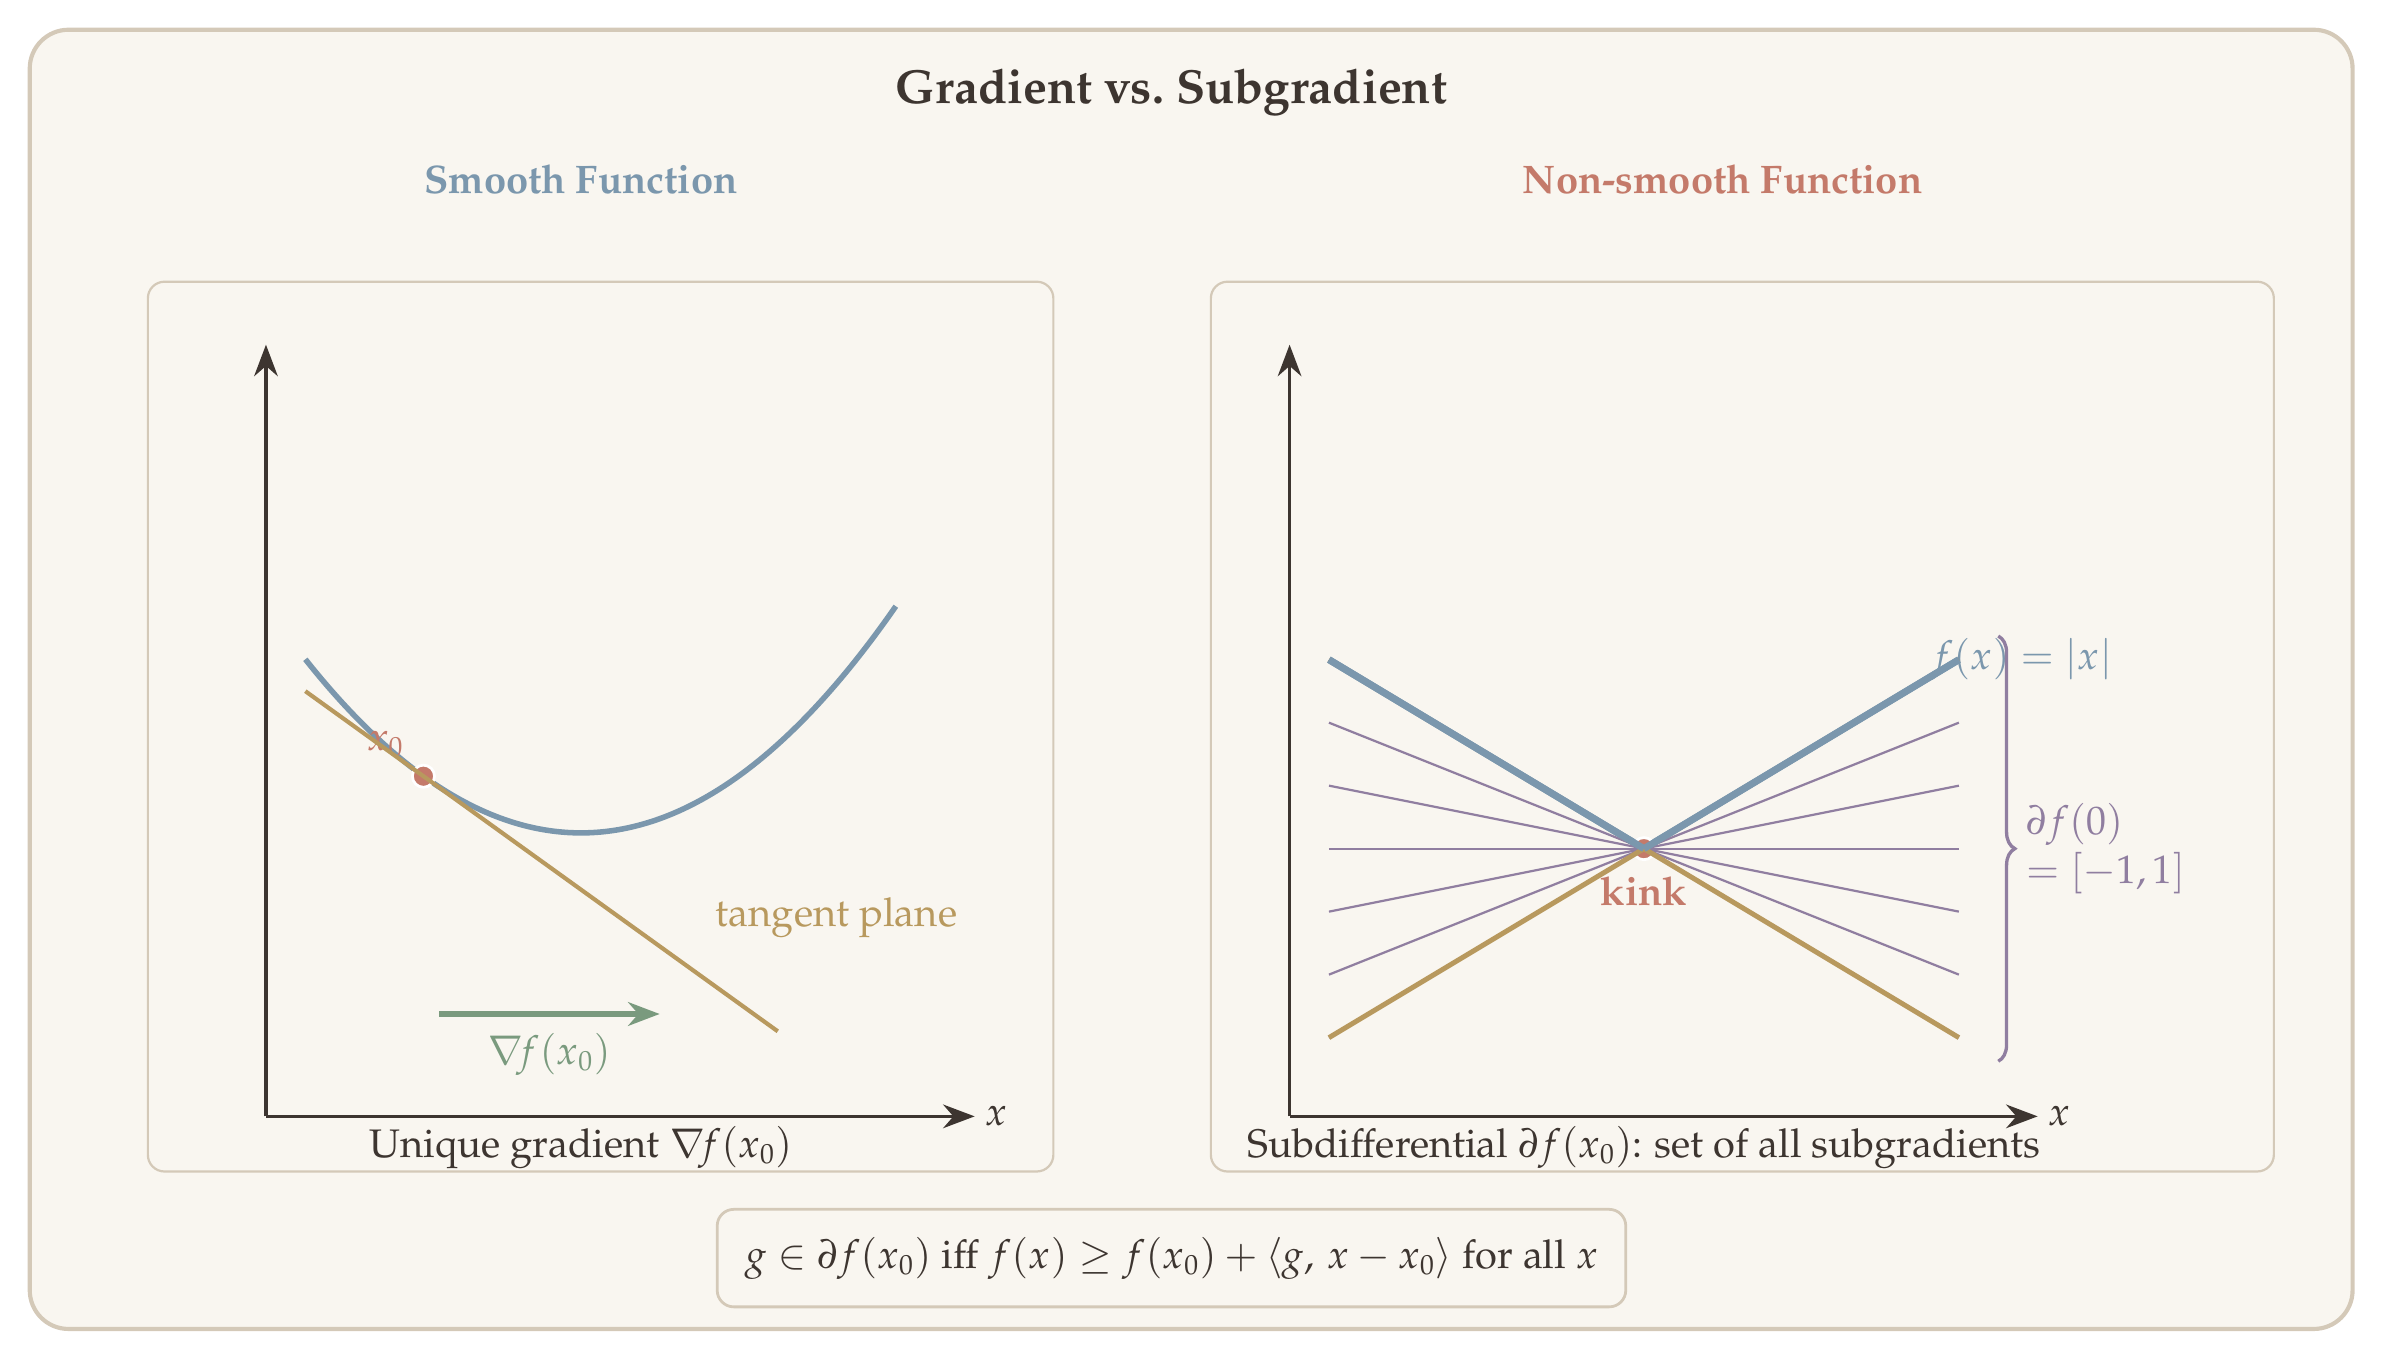
\begin{tikzpicture}[>={Stealth[length=4mm, width=3mm]}, line width=1.5pt]

% Background
\fill[cream, rounded corners=14pt] (-3.0,-5.5) rectangle (26.5,11.0);
\draw[border, line width=1.5pt, rounded corners=14pt] (-3.0,-5.5) rectangle (26.5,11.0);

% Title
\node[font=\LARGE\bfseries, text=dkbrown] at (11.5,10.2) {Gradient vs.\ Subgradient};

% =========== LEFT PANEL: Smooth function ===========
\node[font=\Large\bfseries, text=stblue] at (4.0,9.1) {Smooth Function};

\draw[border, line width=0.8pt, rounded corners=6pt] (-1.5,-3.5) rectangle (10.0,7.8);

% Axes
\draw[->, dkbrown, line width=1.2pt] (0,-2.8) -- (9.0,-2.8)
  node[right, font=\Large, text=dkbrown] {$x$};
\draw[->, dkbrown, line width=1.2pt] (0,-2.8) -- (0,7.0);

% Smooth convex function
\draw[stblue, line width=2pt, smooth, samples=80, domain=0.5:8.0]
  plot (\x, {0.18*(\x-4.0)*(\x-4.0) + 0.8});

% Point of tangency at x=2
\pgfmathsetmacro{\xpt}{2.0}
\pgfmathsetmacro{\ypt}{0.18*(\xpt-4.0)*(\xpt-4.0) + 0.8}
\fill[terracotta] (\xpt, \ypt) circle (4pt);
\draw[white, line width=1pt] (\xpt, \ypt) circle (4pt);
\node[font=\Large\bfseries, text=terracotta, above left=3pt] at (\xpt, \ypt) {$x_0$};

% Tangent hyperplane
\pgfmathsetmacro{\slope}{0.36*(\xpt-4.0)}
\draw[rwgold, line width=1.5pt, domain=0.5:6.5]
  plot (\x, {\ypt + \slope*(\x-\xpt)});
\node[font=\Large, text=rwgold, below right=2pt] at (5.5,0.2) {tangent plane};

% Gradient arrow
\draw[->, sage, line width=2.5pt] (2.2, -1.5) -- (5.0, -1.5);
\node[font=\Large, text=sage, below=3pt] at (3.6, -1.5) {$\nabla\!f(x_0)$};

% Caption
\node[font=\Large, text=dkbrown, align=center] at (4.0,-3.2)
  {Unique gradient $\nabla\!f(x_0)$};

% =========== RIGHT PANEL: Non-smooth function ===========
\node[font=\Large\bfseries, text=terracotta] at (18.5,9.1) {Non-smooth Function};

\draw[border, line width=0.8pt, rounded corners=6pt] (12.0,-3.5) rectangle (25.5,7.8);

% Axes
\draw[->, dkbrown, line width=1.2pt] (13.0,-2.8) -- (22.5,-2.8)
  node[right, font=\Large, text=dkbrown] {$x$};
\draw[->, dkbrown, line width=1.2pt] (13.0,-2.8) -- (13.0,7.0);

% |x| function: f(x) = |x - 17.5| scaled
\pgfmathsetmacro{\kinkx}{17.5}
\pgfmathsetmacro{\kinky}{0.6}
\pgfmathsetmacro{\abslope}{0.6}
\draw[stblue, line width=2.5pt, domain=13.5:\kinkx]
  plot (\x, {-\abslope*(\x-\kinkx) + \kinky});
\draw[stblue, line width=2.5pt, domain=\kinkx:21.5]
  plot (\x, {\abslope*(\x-\kinkx) + \kinky});

\node[font=\Large, text=stblue, right] at (21.0,3.0) {$f(x)=|x|$};

% Kink point
\fill[terracotta] (\kinkx, \kinky) circle (4pt);
\draw[white, line width=1pt] (\kinkx, \kinky) circle (4pt);
\node[font=\Large\bfseries, text=terracotta, below=6pt] at (\kinkx, \kinky) {kink};

% Subdifferential: several supporting hyperplanes
\foreach \s in {-0.6, -0.4, -0.2, 0, 0.2, 0.4, 0.6} {
  \draw[lavender, line width=0.8pt, domain=13.5:21.5]
    plot (\x, {\kinky + \s*(\x-\kinkx)});
}

% Highlight the boundary slopes (match function slopes)
\draw[rwgold, line width=1.8pt, domain=13.5:21.5]
  plot (\x, {\kinky + (-\abslope)*(\x-\kinkx)});
\draw[rwgold, line width=1.8pt, domain=13.5:21.5]
  plot (\x, {\kinky + \abslope*(\x-\kinkx)});

% Redraw function on top
\draw[stblue, line width=2.5pt, domain=13.5:\kinkx]
  plot (\x, {-\abslope*(\x-\kinkx) + \kinky});
\draw[stblue, line width=2.5pt, domain=\kinkx:21.5]
  plot (\x, {\abslope*(\x-\kinkx) + \kinky});

% Subdifferential brace (inside the panel)
\pgfmathsetmacro{\bx}{22.0}
\pgfmathsetmacro{\btop}{\kinky+\abslope*(\bx-\kinkx)}
\pgfmathsetmacro{\bbot}{\kinky-\abslope*(\bx-\kinkx)}
\draw[decorate, decoration={brace, amplitude=6pt}, lavender, line width=1.2pt]
  (\bx, \btop) -- (\bx, \bbot);
\node[font=\Large, text=lavender, right=6pt, align=left] at (\bx,\kinky)
  {$\partial f(0)$\\$= [-1,1]$};

% Caption
\node[font=\Large, text=dkbrown, align=center] at (17.5,-3.2)
  {Subdifferential $\partial f(x_0)$: set of all subgradients};

% =========== Bottom annotation box ===========
\node[text=dkbrown, font=\Large,
      fill=cream, inner sep=10pt,
      draw=border, line width=1pt, rounded corners=6pt]
  at (11.5,-4.6)
  {$g \in \partial f(x_0)$ iff $f(x) \geq f(x_0) + \langle g,\, x - x_0 \rangle$ for all $x$};

\end{tikzpicture}
\end{document}
